\cite{hal02158423}

Zu Grunde liegender Sinn dieses Schrittes: Vertauschen der Anfangswerte, die 
verteilt sind wie $BlueNoise_{t}$, sodass Sie verteilt sind wie die 
$BlueNoise_{t+1}$. Aufgrund dessen haben wir eine Aufsummierung der
blue noise Fehlerverteilungen über viele Frames.

\begin{algorithm}[H]
    \caption{\textbf{Retargeting Schritt} t Vor Rendern Frame t+1 nach Sortier Schritt}
    \begin{algorithmic}[1]
        \State //permutation indices from precomputed texture
        \State $retaget_{t}$ = retargettexure[calcCorrectOffset(incomingbluenoisetexture)];
        \State List<PixelPermutation> L = $retaget_{t}$
        \For{i = 1 .. numberOfPixelsPerBlock}
        \State $retargetedSeeds(L.getNewIndices()) = incomingSeeds(L.getOldIndices());$
        \EndFor
    \end{algorithmic}
    \label{alg:retargetingAlg}
\end{algorithm}

\begin{figure}[H]\label{pic:Permutation}
    \centering
    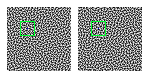
\includegraphics[width=0.5\linewidth]{content/simulatedAnnealing/Bilder/Permutation.png}
    \caption{Permutation}
\end{figure}

%%%%%%%%%%%%%%%%%%%%%%%%%%%%%%%%%%%%%%%%%%%%%%%%%%%%%%%%%%%%
%%%%%%%%%% Beginning the Sequence of getting to blue noise from white noise
%%%%%%%%%%%%%%%%%%%%%%%%%%%%%%%%%%%%%%%%%%%%%%%%%%%%%%%%%%%%

\begin{figure}[H]

    \begin{subfigure}{\textwidth}
        \centering 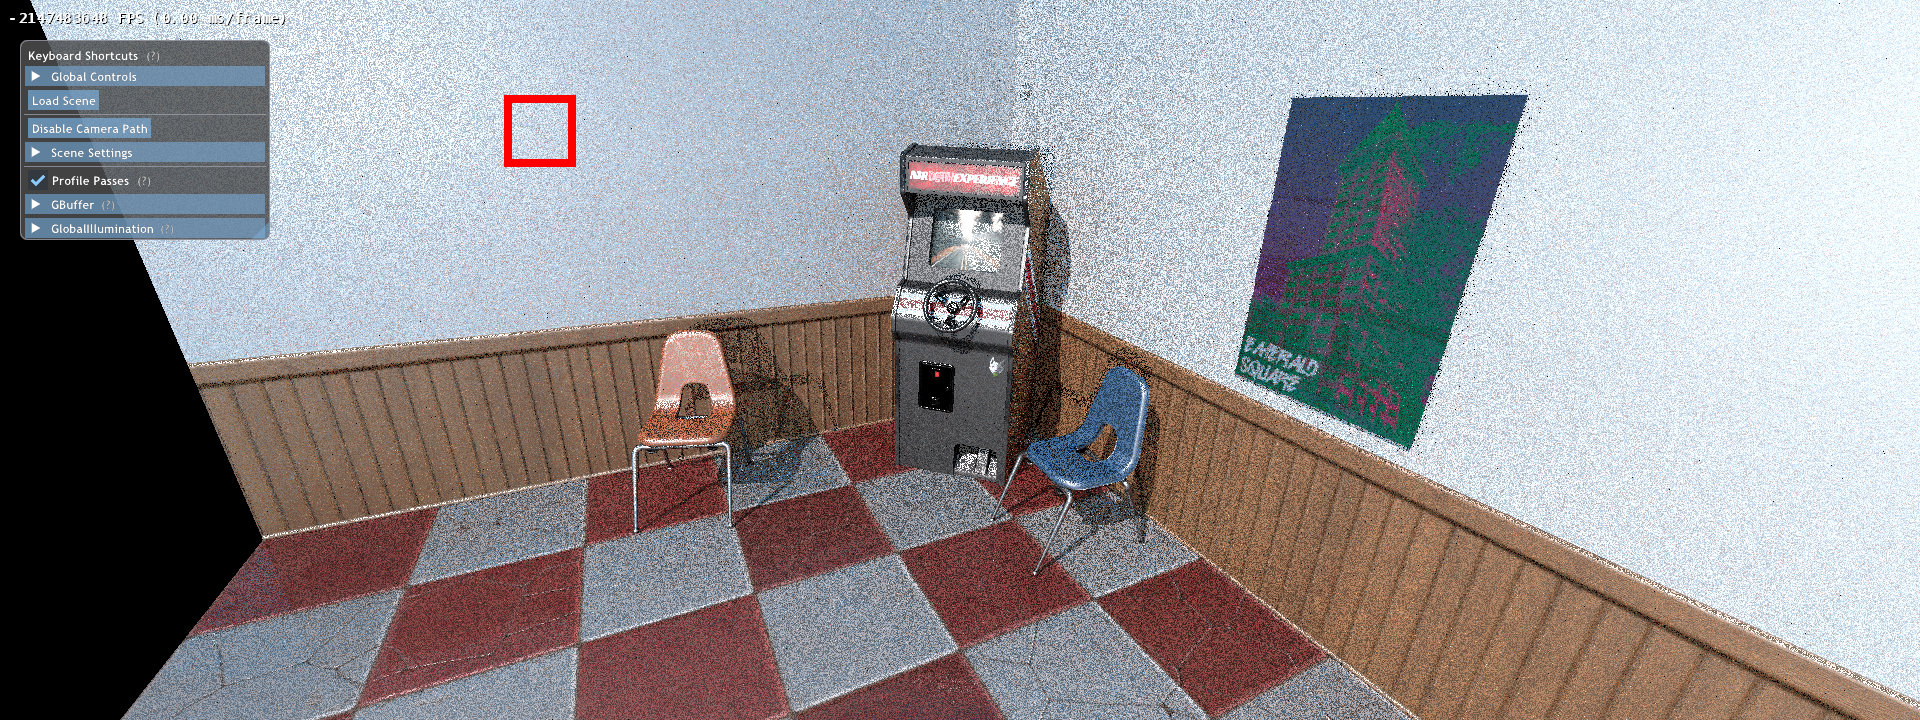
\includegraphics[scale=.2]{content/TemporalerAlg/Bilder/Screenshotreihe/frame_t_2.0.png}
        \caption{Szene}
        \label{fig:Szene_t1}
    \end{subfigure}
    \begin{subfigure}{0.5\textwidth}
        \centering 
\includegraphics[width=0.5\linewidth]{content/TemporalerAlg/Bilder/Screenshotreihe/frame_t_2.0_64x64.png} 
        \caption{Szenenausschnitt}
        \label{fig:ausschnitt_t1}
    \end{subfigure}
    \begin{subfigure}{0.5\textwidth}
        \centering 
\includegraphics[width=0.5\linewidth]{content/TemporalerAlg/Bilder/Screenshotreihe/spektrum/frame_t_2.0_64x64_fourier.png}
        \caption{Fouriertransformierte des Ausschnitts}
        \label{fig:Fouriertransformierte_t1}
    \end{subfigure}
        \caption{Zeitpunkt t=1}
        \label{fig:Verlauf_t1}
\end{figure}

\begin{figure}[H]
    \begin{subfigure}{\textwidth}
        \centering 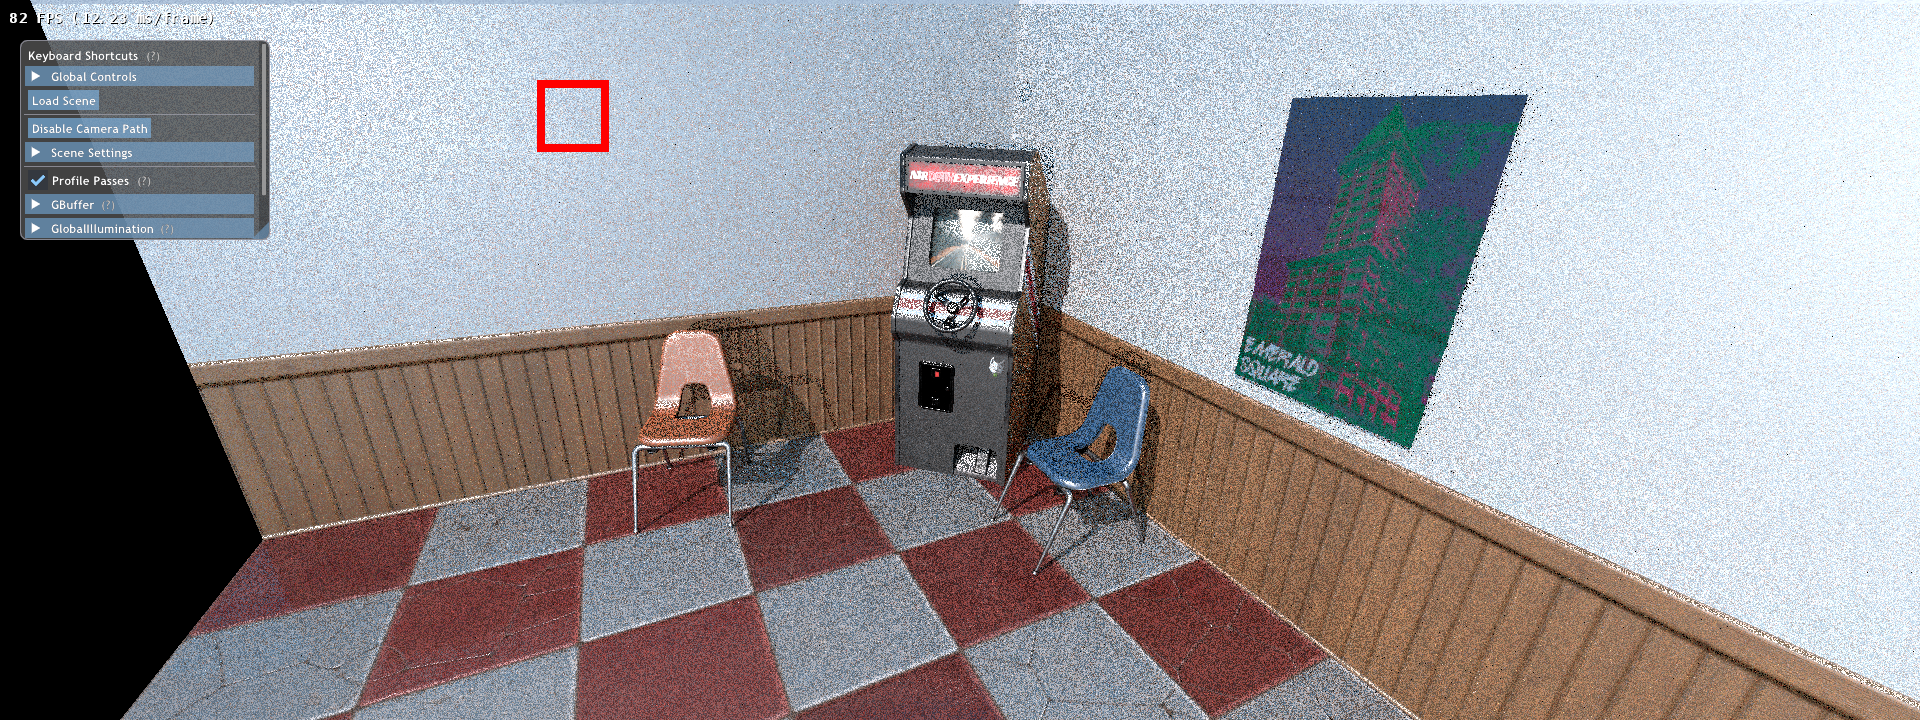
\includegraphics[scale=.2]{content/TemporalerAlg/Bilder/Screenshotreihe/frame_t_3.0.png}
        \caption{Szene}
        \label{fig:Szene_t1}
    \end{subfigure}
    \begin{subfigure}{0.5\textwidth}
        \centering
\includegraphics[width=0.5\linewidth]{content/TemporalerAlg/Bilder/Screenshotreihe/frame_t_3.0_64x64.png} 
        \caption{Szenenausschnitt}
        \label{fig:ausschnitt_t2}
    \end{subfigure}
    \begin{subfigure}{0.5\textwidth}
        \centering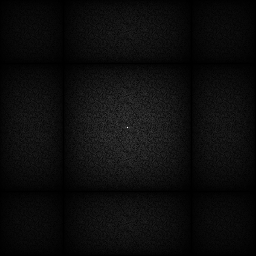
\includegraphics[width=0.5\linewidth]{content/TemporalerAlg/Bilder/Screenshotreihe/spektrum/frame_t_3.0_64x64_fourier.png}
        \caption{Fouriertransformierte des Ausschnitts}
        \label{fig:Fouriertransformierte_t2}
    \end{subfigure}
        \caption{Zeitpunkt t=2}
        \label{fig:Verlauf_t2}
\end{figure}

\begin{figure}[H]
    \begin{subfigure}{\textwidth}
        \centering 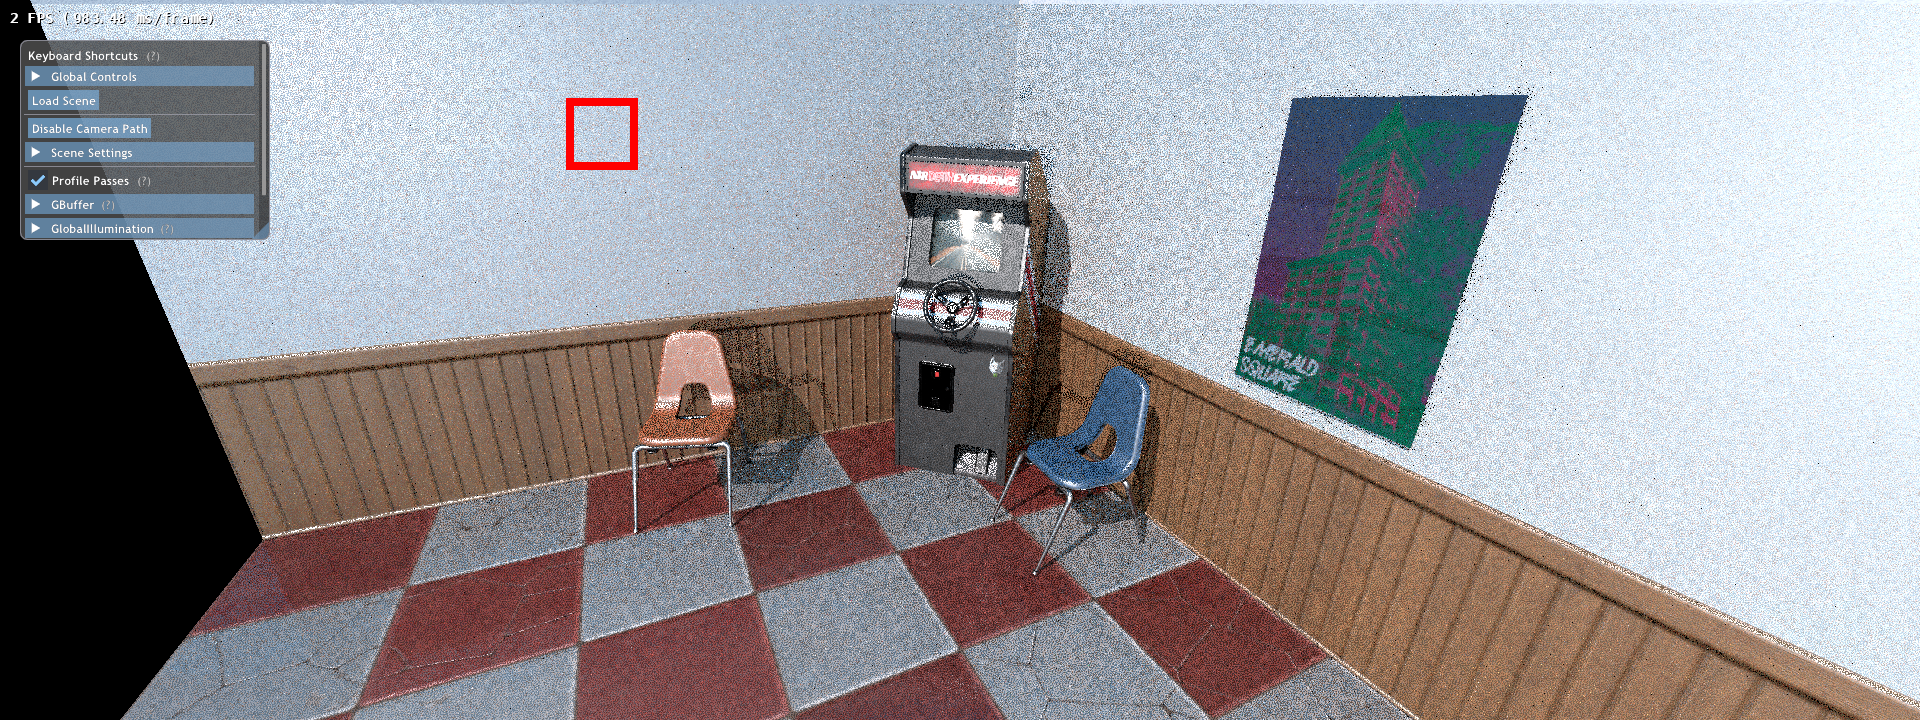
\includegraphics[scale=.2]{content/TemporalerAlg/Bilder/Screenshotreihe/frame_t_4.0.png}
        \caption{Szene}
        \label{fig:Szene_t1}
    \end{subfigure}
    \begin{subfigure}{0.5\textwidth}
        \centering
\includegraphics[width=0.5\linewidth]{content/TemporalerAlg/Bilder/Screenshotreihe/frame_t_4.0_64x64.png} 
        \caption{Szenenausschnitt}
        \label{fig:ausschnitt_t3}
    \end{subfigure}
    \begin{subfigure}{0.5\textwidth}
        \centering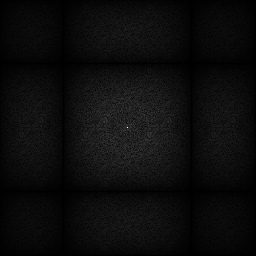
\includegraphics[width=0.5\linewidth]{content/TemporalerAlg/Bilder/Screenshotreihe/spektrum/frame_t_4.0_64x64_fourier.png}
        \caption{Fouriertransformierte des Ausschnitts}
        \label{fig:Fouriertransformierte_t3}
    \end{subfigure}
        \caption{Zeitpunkt t=3}
        \label{fig:Verlauf_t3}
\end{figure}

\begin{figure}[H]
    \begin{subfigure}{\textwidth}  
        \centering 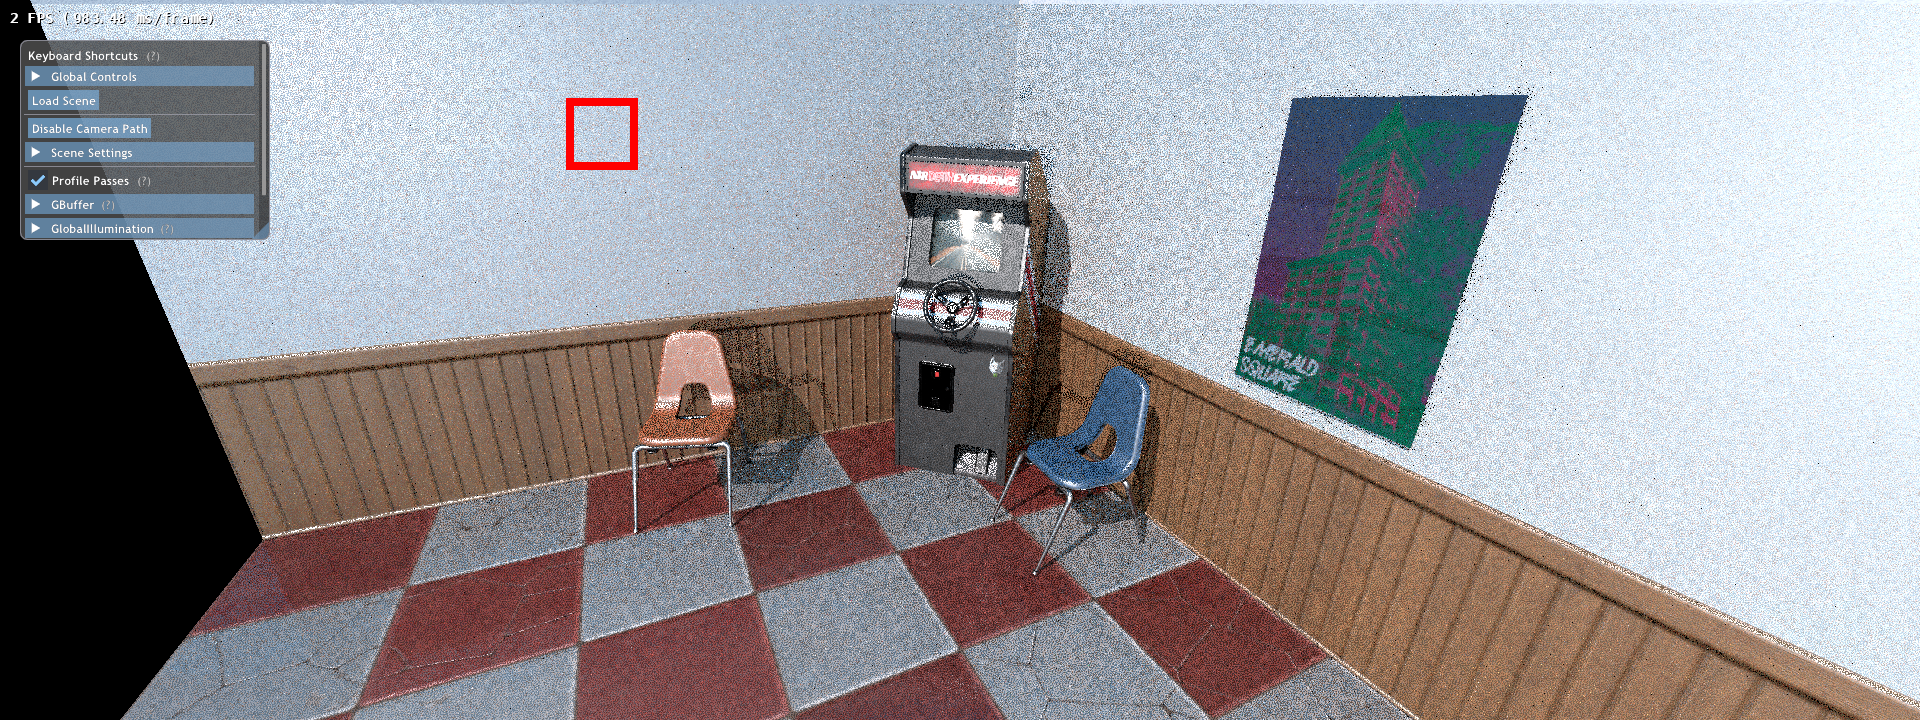
\includegraphics[scale=.2]{content/TemporalerAlg/Bilder/Screenshotreihe/frame_t_4.0.png}
        \caption{Szene}
        \label{fig:Szene_t1}
    \end{subfigure}
    \begin{subfigure}{0.5\textwidth}
        \centering
\includegraphics[width=0.5\linewidth]{content/TemporalerAlg/Bilder/Screenshotreihe/frame_t_4.0_64x64.png} 
        \caption{Szenenausschnitt}
        \label{fig:ausschnitt_t4}
    \end{subfigure}
    \begin{subfigure}{0.5\textwidth}
        \centering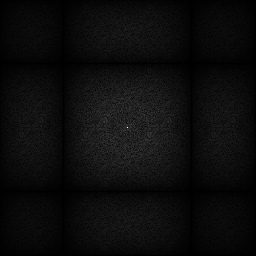
\includegraphics[width=0.5\linewidth]{content/TemporalerAlg/Bilder/Screenshotreihe/spektrum/frame_t_4.0_64x64_fourier.png}
        \caption{Fouriertransformierte des Ausschnitts}
        \label{fig:Fouriertransformierte_t4}
    \end{subfigure}
        \caption{Zeitpunkt t=4}
        \label{fig:Verlauf_t4}
\end{figure}

\begin{figure}[H]
    \begin{subfigure}{\textwidth}   
        \centering 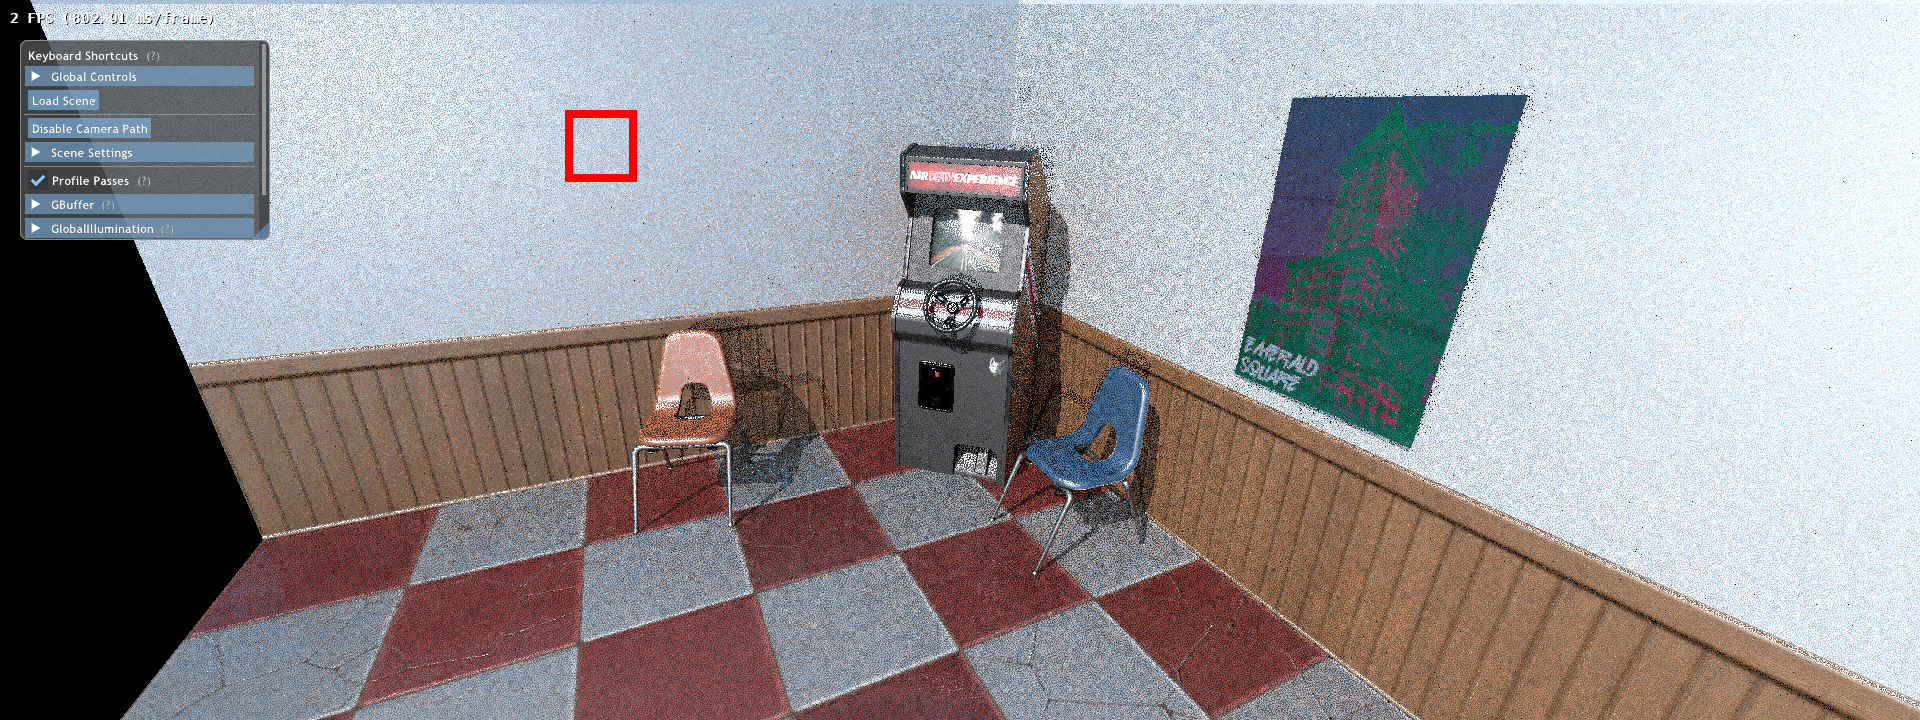
\includegraphics[scale=.2]{content/TemporalerAlg/Bilder/Screenshotreihe/frame_t_5.0.png}
        \caption{Szene}
        \label{fig:Szene_t1}
    \end{subfigure}
    \begin{subfigure}{0.5\textwidth}
        \centering
\includegraphics[width=0.5\linewidth]{content/TemporalerAlg/Bilder/Screenshotreihe/frame_t_5.0_64x64.png} 
        \caption{Szenenausschnitt}
        \label{fig:ausschnitt_t5}
    \end{subfigure}
    \begin{subfigure}{0.6\textwidth}
        \centering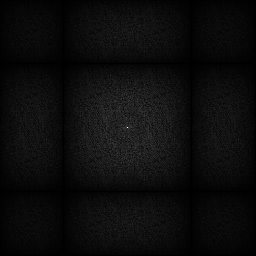
\includegraphics[width=0.5\linewidth]{content/TemporalerAlg/Bilder/Screenshotreihe/spektrum/frame_t_5.0_64x64_fourier.png}
        \caption{Fouriertransformierte des Ausschnitts}
        \label{fig:Fouriertransformierte_t5}
    \end{subfigure}
        \caption{Zeitpunkt t=5}
        \label{fig:Verlauf_t5}
\end{figure}

